\section{安装必备的应用软件}
\subsection{安装及配置Chrome浏览器}
(1) 添加chrome的源

\verb"$ sudo vim /etc/apt/menu.lst"

(2) 添加如下源到文件menu.lst
\begin{verbatim}
deb http://ppa.launchpad.net/fta/ppa/ubuntu karmic main
deb-src http://ppa.launchpad.net/fta/ppa/ubuntu karmic main
\end{verbatim}

(3) 导入密钥
\begin{verbatim}
gpg --keyserver keyserver.ubuntu.com --recv 0c713da6
gpg --export --armor 0c713da6 | sudo apt-key add -
\end{verbatim}

(4) 更新源

\verb"$ sudo apt-get update"

(5) 安装

\verb"$ sudo apt-get install chromium-browser"

此时,chrome浏览器安装完成,但flash仍然无法播放,需要安装flashplayer插件

(6) 如果系统还没安装flashplayer plugin,先安装其:

\verb"$ sudo apt-get install flashplugin-installer"

(7) 将插件拷贝到chrome插件的目录下

\verb"$ sudo cp /usr/lib/flashplugin-installer/libflashplayer.so /usr/lib/chromium-browser/plugins/"

(8) 设置chrome启动时加载插件,修改快捷方式的启动命令为:

\verb"$ sudo chromium-browser %U --enable-extensions --enable-plugins"

(9) 此时,可以播放flash来,但遇到中文字符是乱码,解决方案如下:

\verb"$ sudo vim /etc/fonts/conf.d/49-sansserif.conf"

将edit标签下的sans-serif修改为sans,保存并退出。

(10) Chrome下载文件名出现乱码解决办法:

扳手-------->Settings(设置)-------->ShowAdvance Settings(显示高级设置)-------->Web Content(网页内容)-------->Customizefonts(自定义字体)-------->Encoding(编码)-------->会发现默认设置的是ISO-8859-1-------->现在把它设置成Chinese Simplified(GBK)(中文简体 GBK)-------->你也可以设置自己喜欢的字体-------->问题解决。

\subsection{安装Adobe Reader}
(1)双击下载的安装文件即可完成安装

(2)添加中文支持:

下载font pack包并解压,在目录中运行

\verb"$ sudo sh ./INSTALL"

按提示操作,注意Acrobat Reader 9的安装目录是/opt/Adobe,在输入该目录时只需要输入/opt即可。安装非常简易。安装完成以后便可以打开中文文档。
		
(3)解决PDF阅读器的乱码问题

\subsection{安装China Union 3G驱动}

\subsection{安装EIOffice}

\subsection{安装ibus}
(1) 只需要打开console,输入ibus-daemon -x -r -d就行 

(2) 另外,建议将ibus设置为默认输输入法:

\verb"$ im-switch -s ibus -z default"

(3) 并且默认启动:

系统设置-高级-自动启动,添加程序,输入 ibus-daemon -x -r -d ,确定,最后注销重登。

(4) 如果输入法没有输入框,请检查是否已经安装了 python-notify 包:

\verb"$ sudo apt-get install python-notify"

然后注销重新进入即可。

\subsection {安装INode软件}
(1) 追加可执行权限

\verb"$ sudo chmod –R 777 iNodeClient"

(2) 安装软件

\verb"$ sudo ./install.sh"

(3) 对于ubuntu 12.04还需要安装以下软件:
\begin{verbatim}
# ln –s /usr/lib/i386-linux-gnu/libtiff.so.4 /usr/lib/i386-linux-gnu/libtiff.so.3
# apt-get install libjpeg62
\end{verbatim}

\subsection{安装Picasa}

\subsection{安装ppstream}

\subsection{安装牛津高阶词典}
最近一直在用ubuntu系统在看英文pdf书籍,可是在linux安装的词典,对词条解释的太麻烦,而且有不可发音。因为学习上的需要,所以自己要安装 个牛津词典。之所以发表这个博客是想告诉大家如何简单的在ubuntu安装词典,自己在安装时候也看了过网上的安装方法,但是比较复杂,而且也不能发音,所 以希望这篇博文能给安装oald8带来方便

1:下载词典

牛津高阶词典下载地址:http://www.verycd.com/topics/2808053/

2:提取文件

在windows下建立一个新的文件夹oxford,然后将oald8.iso文件用虚拟光驱以文件形式的打开,打开后将里面的文件都复制的新建的oxford中。

3:启动ubuntu系统

在windows下建立一个新的文件夹oxford,然后将oald8.iso文件用虚拟光驱以文件形式的打开,打开后将里面的文件都复制的新建的oxford中。如图\ref{oxford}所示:
\begin{figure}
\centering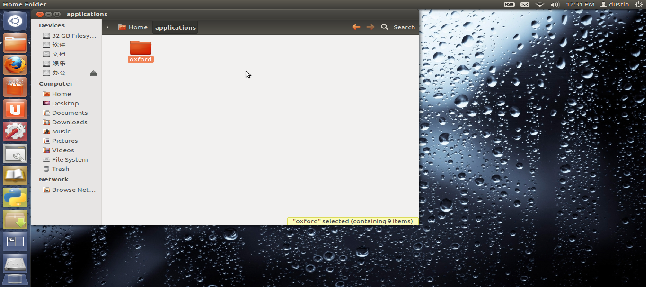
\includegraphics[scale=0.7]{figures/oxford.png}
\caption{安装词典}\label{oxford}
\end{figure}


双击oxford文件夹,然后在打开linux文件夹,发现里面有一个setup.sh,右击setup.sh选择属性,点击权限设置,选择Allow excuting file as program。

4:安装牛津高阶英语词典

Alt+Ctrl+T打开终端,用cd命令打开setup.sh所在的文件夹。然后输入 ./setup.sh(安装词典的意思)

5:安装过程设置

按回车就可以继续下一步

是否同意安装

安装结束

安装的过程可以自己设置安装路径,也可按照软件提供的路径。要是选择第二种话,安装过程一直按'回车'就可以的。

6:启动快捷方式设置

并不是安装结束后,这个软件就可以运行了,还需要下面关键两个步骤!

1:启动设置:

将快捷方式设置成可执行程序,否则在双击这个快捷方式,是不能执行的, 所以也就不能启动oald8软件了。右击桌面快捷方式,选择属性,权限设置,将这个快捷方式设置成可执行程序。

2:词典发音设置:

若是没有这步骤,词典是不可发音的,具体过程如下:

command设置,这个也是很关键一步,若是不设置这个command,这个软件  是不能发音的。同样是右击桌面的快捷方式,选择属性,你会发现有command里写着的是:home/dustin/oald8//oald8将其改为如下命令:    padsp '/home/dustin/oald8//oald8',这个命令要根据安装路径的不同还有用户名字而定,写一个通用的命令吧,自己要根据自己的用户名,还有安装路径自己设置吧padsp '/home/用户名字/安装路径//oald8'

最后大家就可以使用这个很棒的牛津词典了,perfect!

\subsection{安装Dropbox}
1. Add Dropbox’s repository key

\verb"$ sudo apt-key adv --keyserver pgp.mit.edu --recv-keys 5044912E"

2. Add Dropbox’s repository
\begin{verbatim}
$ sudo add-apt-repository "deb http://linux.dropbox.com/ubuntu $(lsb_release -sc) main"
\end{verbatim}

3. update and install Dropbox

\begin{verbatim}
$ sudo apt-get update"
$ sudo apt-get install dropbox nautilus-dropbox
\end{verbatim}

4. Follow the steps When dropbox prompted with the screen

\subsection{安装Skype}
\begin{verbatim}
sudo apt-add-repository "deb http://archive.canonical.com/ $(lsb_release -sc) partner"
sudo apt-get update && sudo apt-get install skype
\end{verbatim}

\subsection{安装图片编辑工具gimp}
\verb"$ sudo apt-get install gimp"

\subsection{安装电驴下载软件amule}
\verb"$ sudo apt-get install amule"

\subsection{smaplyer}
\verb"$ sudo apt-get install smplayer subdownloader"

播放文件时标题栏经常会出现乱码,解决办法:

首选项—>高级—>在窗口标题上显示标签信息这一项去掉,smplayer标题栏显示的就是你的文件名了。

\subsection{ubuntu one}

\subsection{下载youtube视频}
(1) 用下列指令安裝youtube-dl

\verb"$ sudo apt-get install youtube-dl"

(2) 用瀏覽器瀏覽http://youtube.com,搜尋到需要的影片後複製其網址

輸入下列指令先找出能下載的影片格式,我打算下載成1080p的高清格式,因此格式代碼是137(後記:137、136下載的檔案都無法播放,改用22就可以):
\verb"$ youtube-dl -F http://www.youtube.com/watch?v=7pKHsPcQot4"
\begin{figure}
\centering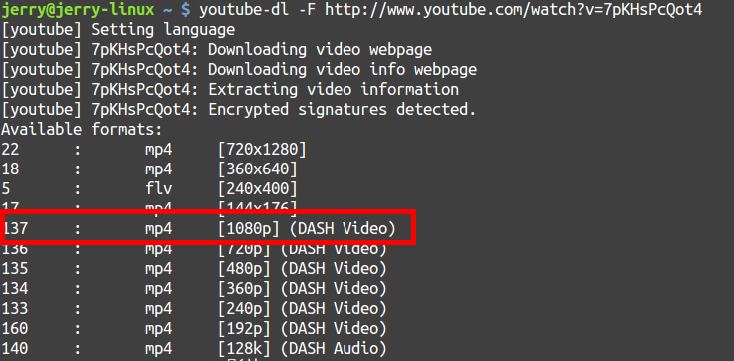
\includegraphics[scale=0.5]{figures/youtube.png}
\caption{youtube可用参数}\label{youtube1}
\end{figure} 
(3) 以-f 137下載成1080p的格式:

\verb"$ youtube-dl -f 137 http://www.youtube.com/watch?v=7pKHsPcQot4"
\begin{figure}
\centering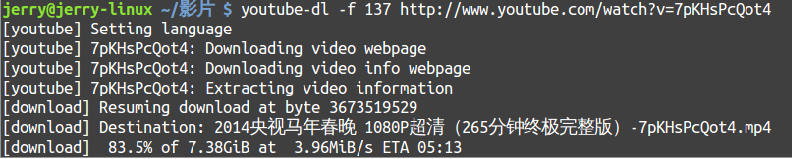
\includegraphics[scale=0.5]{figures/youtube1.png}
\caption{youtube使用举例}\label{youtube2}
\end{figure} 

\subsection{一个Linux脚本搞定常用软件的安装}
\begin{verbatim}
  #Bittorrent
  sudo apt-get remove bittorrent -y
  #安装StarDict翻译词典
  sudo apt-get install stardict stardict-common  --force-yes -y
  sudo apt-get install stardict-cdict-gb stardict-cedict-gb stardict-hanzim stardict-langdao-ce-gb stardict-langdao-ec-gb stardict-oxford-gb stardict-xdict-ce-gb stardict-xdict-ec-gb  --force-yes -y
  #安装浏览器Flash插件:
  sudo mkdir -p /usr/lib/X11/fonts/Type1
  sudo apt-get install flashplugin-nonfree --force-yes -y
  #安装FTP工具
  sudo apt-get install gftp --force-yes -y
  #安装进入终端的右键快捷菜单
  sudo apt-get install nautilus-open-terminal --force-yes -y
  #alien--把rpm包转换成deb包。使用命令:alien abc.rpm
  sudo apt-get install alien --force-yes -y
  #安装视频播放软件和相应解码器
  sudo apt-get install mplayer mozilla-mplayer libxine-extracodecs w32codecs --force-yes -y
  sudo apt-get install gstreamer0.10-plugins-ugly gstreamer0.10-pitfdll gstreamer0.10-ffmpeg --force-yes -y
  sudo apt-get install im-switch fcitx libapt-pkg-perl --force-yes -y
  #切换输入法
  sudo im-switch -s fcitx
  #阅读CHM文件,chmsee对某些不规范的chm文件支持效好, gnochm支持搜索
  sudo apt-get install chmsee gnochm --force-yes -y
  #桌面搜索,功能类似于GOOGLE的那个桌面搜索。安装后在“附件”菜单可找到一个“搜索”项
  sudo apt-get install beagle --force-yes -y
  sudo apt-get install gnuplot vim automake autoconf  gwenview kchmviewer alien nautilus-open-terminal
\end{verbatim}

\subsection{安装压缩解压缩}
\verb"$ sudo apt-get install unace unrar zip unzip p7zip-full p7zip-rar sharutils rar uudeview mpack lha arj cabextract"

\subsection{安装vlc视频播放器}
(1) 音视频播放:

\verb"$ sudo apt-get install vlc"

(2) 安装编解码器:

\verb"$ sudo apt-get install non-free-codecs libxine1-ffmpeg gxine mencoder libmpcdec3 libquicktime1 flac faac faad sox ffmpeg2theora libmpeg2-4 uudeview flac libmpeg3-1 mpeg3-utils mpegdemux liba52-dev mpeg2dec vorbis-tools id3v2 mpg321 mpg123 libflac++6 ffmpeg libmp4v2-0 totem-mozilla icedax tagtool easytag id3tool lame nautilus-script-audio-convert libmad0 libjpeg-progs"

\subsection{安装WPS办公软件}
(1) 将下载的WPS和symbol font的deb文件双击安装即可。

(2) 将下载的字体文件解压缩到~/.fonts目录即可解决字体丢失问题

\subsection{修改系统的默认字体}
(1) 左键点击右上角的齿轮,找到其中的系统设置选项.

(2) 点击universal access, 在contrast下拉列表中选择small即可.

\subsection{修改系统输入法}
(1) 按一下windows键然后在出现的对话框中输入keyboard命令并找到图标点击.

(2) 点击OK后出现的对话框中运行相应的设置即可.

(3) 添加五笔输入法:
\verb"$ sudo apt-get install ibus-table-wubi"

(4) 点击右上角的齿轮,选择startup applications.在弹出来的对话框的command里填写/usr/bin/ibus-daemon –d, Name和commer可乱写.

\subsection{BT下载工具}
\verb"$ sudo apt-get install deluge"

\subsection{系统配置工具}
(1) 安装编辑器配置工具

\verb"$ sudo apt-get install myunity gconf-editor dconf-tools"

(2) 安装ubuntu-tweak
\begin{verbatim}
# apt-add-repository ppa:tualatrix/ppa
# apt-get update
# apt-get install ubuntu-tweak
\end{verbatim}

\subsection{安装QQ软件}
(1) 安装QQ软件

\verb"$ sudo dpkg –I WineQQ2013.deb"

(2) 配置ibus输入法

在/etc/profile文件最后添加
\begin{verbatim}
XMODIFIERS="@im=ibus"
XIM="ibus"
GTK_IM_MODULE="xim"
QT_IM_MODULE="xim"
ibus-daemon -d –x
把/etc/X11/xinit/xinput.d/ibus 文件中的 XIM_ARGS="--xim" 改成XIM_ARGS="-d -x"
\end{verbatim}

\subsection{安装dock工具}
\verb"$ sudo apt-get install docky cairo-dock conky screenlets"

\subsection{gmail邮件通知工具}
\verb"$ sudo apt-get install gm-notify"

\subsection{Liberoffice的美化工具}
\verb"$ sudo apt-get install lo-menubar"

\subsection{解除gedit乱码}
(1) apt-get install dconf-tools

(2) 在终端输入dconf-editor

(3) 找到org-gnome-gedit-preferences-encodings在其中UTF-8前面添加’GBK’就可以了.

也可以命令行下输入:
\begin{verbatim}
  gsettings set org.gnome.gedit.preferences.encodings \ 
  auto-detected "['UTF-8','GB18030','GB2312','GBK','BIG5','CURRENT','UTF-16']"
\end{verbatim}

\subsection{安装assaultcube游戏软件}
(1) 下载地址http://assault.cubers.net/

(2) 下载解压后点击assaultcube.sh就可以玩咯

\subsection{PDF Xchange}

\subsection{安装thunderbird邮件客户端}
\verb"$ sudo apt-get install thunderbird"

在tool-> add-on中搜索’new mail attention’插件并安装即可收到邮件揭醒。

\subsection{安装115网盘}
